\documentclass{beamer}

\usepackage{xeCJK}
\usepackage{algorithm}  
\usepackage{algorithmic}

\setCJKmainfont[BoldFont = {黑体}]{宋体}
\setlength{\parindent}{22pt}

\usetheme{CambridgeUS}
\usefonttheme{serif}

\title{The Runs Theorem and Lyndon Tree}
\author{杨骏昭、徐翊轩、陈孙立}
\institute{NFLS、SCZ}

\begin{document}

\begin{frame}
    \titlepage
\end{frame}

\begin{frame}{Contents}
	\tableofcontents
\end{frame}

\section{Runs and The Runs Theorem}

\subsection{Preliminaries}

\begin{frame}{Basic Definitions}
    \par \textbf{字符串:}令$\Sigma$为一个有限的有序字符集,一个$\Sigma*$中的元素被称为字符串。我们将字符串$s$的长度表示为$|s|$,定义空串$\epsilon$的长度为0。
    \pause
    \par \textbf{前缀、子串、后缀:}对于字符串$s=xyz$,$x,y,z$分别被称为$s$的一个前缀、子串、后缀。对于$s$的一个前缀$x$,若$x\ne s$,则称$x$是$s$的一个严格前缀,后缀同理。我们用$s[i]$表示字符串$s$的第$i$个字符$(1\leq i\leq |s|)$,用$s[i...j]$表示第$i$个字符和第$j$个字符中间的字符形成的子串$(1\leq i\leq j\leq |s|)$,定义$s[i...j]=\epsilon\ (i>j)$。
	\pause
	\par \textbf{Period:}我们称整数$p$是字符串$s$的period,当且仅当对于任意$1\leq i\leq|s|-p$,$s[i]=s[i+p]$均成立。
	\pause
    \par \textbf{Beg(I):}对于区间集合$I$,定义$Beg(I)$表示$I$中所有区间的起始端点组成的集合。
\end{frame}

\subsection{Runs and Lyndon Words}

\begin{frame}{Runs}
    \par \textbf{定义1\ (Runs):}令字符串$w$的长度为$n$,三元组$r=(i,j,p)$被称为字符串$w$的一个run,当且仅当$w[i...j]$最小的period\ $p$满足$2p\leq |w[i...j]|$,并且该周期性质不可以再向左右延伸,即$i=1$或$w[i-1]\ne w[i+p-1]$,并且$j=n$或$w[j+1]\ne w[j-p+1]$。实数$\frac{j-i+1}{p}$被称为$r$的指数。
    \pause
    \par \textbf{一些关于Runs的符号:}我们用$Runs(w)$来表示$w$中所有的run构成的集合;$\rho(n)$表示长度为$n$的字符串中至多含有的run的个数;$\sigma(n)$表示长度为$n$的字符串中所有run的指数和的最大值。
	\pause
    \par \textbf{字典序:}我们用$<$来表示一个$\Sigma$上的全序关系,并以此定义$\Sigma*$上的字典序关系$<$。
\end{frame}

\begin{frame}{Lyndon Words}
    \par \textbf{定义2\ (Lyndon Word):}非空字符串$w\in\Sigma*$被称为一个关于$<$的Lyndon Word,当且仅当$w<u$对于$w$任意的一个严格后缀$u$都成立。
    \pause
    \par 由Lyndon Word的定义,任意一个Lyndon Word\ $w$都不能具有任何小于$|w|$的period,否则可以导出一个$<w$的严格后缀$u$的存在,与定义不符。
	\pause
    \par \textbf{引理3:}令$w=u^ku'a$,其中$u$为一个Lyndon Word,$u'$为$u$的一个可以为空的严格前缀,$k$为正整数,并且$a\in\Sigma,a\ne w[|u'|+1]$。若$w[|u'|+1]<a$,那么$w$是一个Lyndon Word;否则,即$a<w[|u'|+1]$,那么$u$是任何一个以$w=u^ku'a$为前缀的字符串的最长Lyndon Word前缀。
	\pause
    \par 引理3常被用作字符串的Lyndon分解\footnote{https://loj.ac/problem/129}。证明比较显然,相关证明可以参考Lyndon分解算法。
\end{frame}

\begin{frame}{Lyndon Roots}
    \par \textbf{定义4\ (Lyndon Root):}令$r=(i,j,p)$是字符串$w\in\Sigma*$的一个run,长度为$p$的区间$\lambda=[i_{\lambda}...j_{\lambda}]$被称为$r$关于$<$的Lyndon Root,当且仅当$i\leq i_{\lambda}\leq j_{\lambda}\leq j$,并且$w[i_{\lambda}...j_{\lambda}]$是一个关于$<$的Lyndon Word。
    \pause
    \par 显然,对于任意的一组$r$和$<$,$r$均存在至少一个Lyndon Root。
\end{frame}

\subsection{The Runs Theorem}

\begin{frame}{The Runs Theorem}
    \par 容易发现,在一个一元字符集上的任意一个字符串都只能具有至多一个run,在下面的的讨论中,我们不考虑此类字符串。记$<_0,<_1$为两种相反的$\Sigma$上的全序关系,即对于任意$a,b\in\Sigma$,有$a<_0b\Leftrightarrow b<_1a$,并以此定义$\Sigma*$上的字典序关系$<_0,<_1$。对于$\ell\in\{0,1\}$,令$\bar{\ell}=1-\ell$。对于任意字符串$w\in\Sigma*$,令$\hat{w}=w\$$,其中$\$\notin\Sigma$,是一个特殊字符,满足对于任意$a\in\Sigma$,有$\$<_0a$,$a<_1\$$。
    \pause
    \par \textbf{The Runs Theorem:}$\rho(n)<n,\sigma(n)\leq3n-3$。
\end{frame}

\begin{frame}{Proof}
    \par \textbf{定义5:}对于任意长度为$n$的字符串$w$及其中一个位置$i\ (1\leq i\leq|w|)$,令$l_{\ell}(i)=[i...j]$,其中$j=max\{j'\ |\hat{w}[i...j']$是一个关于$<_{\ell}$的Lyndon Word$\}$。
	\pause
    \par \textbf{引理6:}对于任意长度为$n$的字符串$w$及其中一个位置$i\ (1\leq i\leq|w|)$,有且仅有一个$\ell\in\{0,1\}$,满足$l_{\ell}(i)=[i...i]$,且$l_{\bar{\ell}}(i)=[i...j]\ (j>i)$。
	\pause
    \par \textbf{证明:}令$k=max\{k'\ |\hat{w}[k']\ne \hat{w}[i],k'>i\}$,令$\ell\in\{0,1\}$满足$\hat{w}[k]<_{\ell}\hat{w}[i]$,由\textbf{引理3},$l_{\ell}(i)=[i...i]$,且$l_{\bar{\ell}}(i)=[i...j]\ (j\geq k>i)$。
\end{frame}

\begin{frame}{Proof}
	\par \textbf{引理7:}令$r=(i,j,p)$为长度为$n$的字符串$w$中任意的一个run,那么,有且仅有一个$\ell\in\{0,1\}$满足$\hat{w}[j+1]<_{\ell}\hat{w}[j+1-p]$。所有$r$的关于$<_{\ell}$的Lyndon Root\ $\lambda=[i_{\lambda}...j_{\lambda}]$都与$l_{\ell}(i_{\lambda})$相等。
	\pause
    \par \textbf{证明:}由$r$的定义,$\hat{w}[j+1]\ne\hat{w}[j+1-p]$,因此有且仅有一个$\ell\in\{0,1\}$满足$\hat{w}[j+1]<_{\ell}\hat{w}[j+1-p]$。令$\lambda=[i_{\lambda}...j_{\lambda}]$为$r$的关于$<_{\ell}$的一个Lyndon Root,由\textbf{引理3},$[i_{\lambda}...j_{\lambda}]=l_{\ell}(i_{\lambda})$。
	\pause
    \par 对于字符串$w$中任意的一个run\ $r=(i,j,p)$,令$B_r=\{\lambda=[i_{\lambda}...j_{\lambda}]|\lambda$为$r$的关于$<_{\ell}$的一个Lyndon Root且$i_{\lambda}\ne i\}$,其中$\ell\in\{0,1\}$满足$\hat{w}[j+1]<_{\ell}\hat{w}[j+1-p]$。即$B_r$表示所有$r$的关于$<_{\ell}$的Lyndon Root构成的集合,但要除去开头位置$i$处开始的Lyndon Root(如果它存在的话)。有$|Beg(B_r)|=|B_r|\geq \lfloor e_r-1\rfloor\geq 1$,其中$e_r$为$r$的指数。
\end{frame}

\begin{frame}{Proof}
    \par \textbf{引理8:}对于字符串$w$的两个不同的run\ $r,r'$,$Beg(B_r)\cap Beg(B_{r'})$为空。
	\pause
    \par \textbf{证明:}考虑反证法,假设存在$i\in Beg(B_r)\cap Beg(B_{r'})$,并且$\lambda=[i...j_{\lambda}]\in B_r$,$\lambda'=[i...j_{\lambda'}]\in B_{r'}$。令$\ell\in\{0,1\}$满足$\lambda=l_{\ell}(i)$,由于$\lambda\ne \lambda'$,有$\lambda'=l_{\bar{\ell}}(i)$。由\textbf{引理6},$\lambda$和$\lambda'$中有且只有一个为$[i...i]$。我们不失一般性地假设$\lambda=[i...i]$,那么$j_{\lambda'}>i$。由于$w[i...j_{\lambda'}]$为一个Lyndon Word,有$w[i]\ne w[j_{\lambda'}]$。由$B_r$和$B_{r'}$的定义,$r$和$r'$的开始位置均小于$i$,这意味着$w[i-1]=w[i]$(由$r$的周期性),并且$w[i-1]=w[j_{\lambda'}]$(由$r'$的周期性)。因此我们得到了一对矛盾的结论,假设不成立。
\end{frame}

\begin{frame}{Proof}
    \par \textbf{引理8}表明,任意的一个run\ $r$可以被赋予一个两两不交的非空位置集合$Beg(B_r)$。并且,由于$1\notin Beg(B_r)$对于任意的一个$r$均成立,有$\sum_{r\in Runs(w)}|B_r|=\sum_{r\in Runs(w)}|Beg(B_r)|\leq |w|-1$。因此,我们可以证明如下定理:
	\pause
    \par \textbf{定理9:}$\rho(n)<n$。
	\pause
	\par \textbf{证明:}考虑长度为$n$的字符串$w$,由于对于任意$r\in Runs(w)$,有$|B_r|\geq1$,由\textbf{引理8},有$|Runs(w)|\leq\sum_{r\in Runs(w)}|B_r|\leq n-1$。
	\par \textbf{定理10:}$\sigma(n)\leq3n-3$。
	\pause
	\par \textbf{证明:}考虑长度为$n$的字符串$w$,令$e_r$表示$r$的指数。由于对于任意$r\in Runs(w)$,有$|B_r|\geq \lfloor e_r-1\rfloor>e_r-2$,由\textbf{引理8},有$\sum_{r\in Runs(w)}(e_r-2)<\sum_{r\in Runs(w)}\lfloor e_r-1\rfloor\leq\sum_{r\in Runs(w)}|B_r|\leq n-1$。结合\textbf{引理9}中的$|Runs(w)|\leq n-1$,可得$\sum_{r\in Runs(w)}e_r\leq3n-3$。
	\pause
	\par 至此,The Runs Theorem证明完毕。
\end{frame}

\section{How to compute runs and Lyndon Tree}

\subsection{The algorithm}
\begin{frame}{How to compute Lyndon Roots}
	\par \textbf{引理7}表明,每个run都至少包含一个与$l_{\ell}(i)$相等的Lyndon Root。接下来的算法算出了所有的$l_{\ell}(i)$。
	\pause
	\par \textbf{引理11:}对于任意的两个Lyndon Word $u,v$,且$u<v$,那么$uv$是一个Lyndon Word。
	\pause
	\par \textbf{引理12:}任意字符串$w$都可以被分解成唯一的\textbf{字典序不上升}的Lyndon Word序列$f_1...f_m$,这个序列被称为这个字符串的Lyndon分解。每个$f_i$都是$\overline{f_i...f_m}$的最长Lyndon前缀。
	\pause
	\par \textbf{算法思路:}从右往左对于字符串的每个后缀维护Lyndon分解$f_1...f_m$。每次向左新加一个字符$c$时,将$c$作为一个Lyndon word插入$f$序列的开头,如果序列中存在相邻的两个Lyndon Word $u, v$满足$u<v$,则将$u$和$v$合并为$uv$,直至序列满足字典序不上升为止。由\textbf{引理11和引理12}可知算法正确性。注意只需要比较新加的串与Lyndon分解开头的字符串的字典序大小即可。
	
\end{frame}


\begin{frame}{How to compute Lyndon Roots}
	\par 由于Lyndon串的特殊性质,比较相邻两个Lyndon串字典序的大小关系时可以直接比较它们所代表的后缀的大小关系。虽然它对复杂度分析没有什么影响(可以使用LCP实现比较两个子串大小),但是一定程度上简化了我们的代码。这个性质也揭露下文提到的Lyndon tree的本质。\textbf{引理13}说明了它的正确性。
\end{frame}

\begin{frame}{How to compute Lyndon Roots}
	\par \textbf{引理13:} 对于任意Lyndon串$u$,Lyndon分解$f_1...f_m$,$u<f_1$当且仅当$\overline{u f_1...f_m}<\overline{f_1...f_m}$。
	\pause
	\par \textbf{证明:} 设$v = f_1, u' = \overline{u f_1...f_m}, v' = \overline{f_1...f_m}$。若$u, v$第一个不相同的字母的下标小于等于$min(|u|, |v|)$,那么$u',v'$的大小关系与$u, v$的大小关系相同。我们下面只需要讨论三种情况:$u$是$v$的严格前缀、$v$是$u$的严格前缀、$u$与$v$相等。
	\pause
	\par 若$u$是$v$的严格前缀,那么$u<v$。由于$v$是Lyndon串,所以有$v[1...|v|-|u|]<v[|u|+1...|v|]$,那么$u'<v'$。
	\pause
	\par 若$v$是$u$的前缀,那么$u \ge v$。此时$u, f_1, ... , f_m$为Lyndon分解。所以$u$是$u'$的最长Lyndon前缀。由\textbf{引理3}可得,$u' \ge v'$。
	\pause
	\par 综上所述,$u<v$当且仅当$u'<v'$。
\end{frame}

\begin{frame}{How to compute Lyndon Roots}

\begin{figure}[h]%%图片
	\centering  
	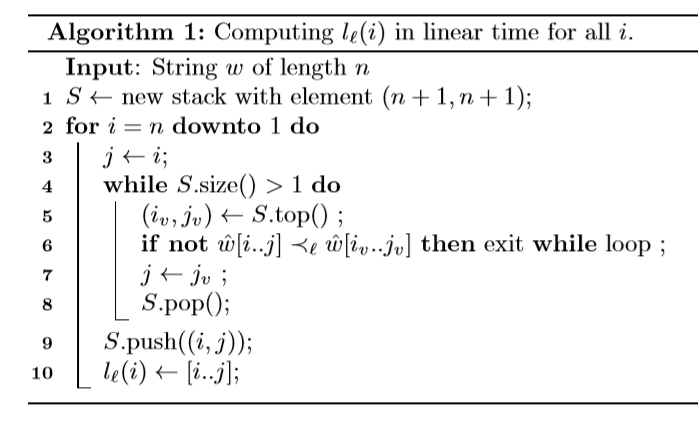
\includegraphics[width=0.7\linewidth]{figures/algorithm.png}
\end{figure}
	\pause
	\par 这个算法用$O(n)$的时间复杂度求出了每个后缀的Lyndon分解,相当于求出了$l_{\ell}(i)$。
	\pause
	\par 可以发现我们实际维护的就是$ISA$数组的单调栈。
\end{frame}

\begin{frame}{How to compute runs}
	\par 枚举$i$,设$l_{\ell}(i)=[l...r]$。我们分别求出最长的$l_1, l_2$使得$w[l...l+l_1-1]=w[r+1...r+l_1]$, $w[l-l_2...l-1]=w[r-l_2...r-1]$。若$l_1+l_2 \ge 2(r-l+1)$,那么我们就找到了一个run,即$(l-l_2, r+l_1-1, r-l+1)$。
	\pause
	\par 这一步其实相当于向前向后求LCP。
	\pause
	\par 注意我们需要先枚举$\ell$,即字典序是顺序还是逆序。
\end{frame}

\begin{frame}{How to compute runs}
	\par \textbf{定理14:} 设$n$为字符串长度。以上算法可以用$O(n)$的时空复杂度找出所有的runs。
	\pause
	\par 使用线性算法(SA-IS)构造后缀数组,并且使用线性预处理$O(1)$询问的RMQ算法来支持LCP询问,整个算法即可做到线性。
	\pause
	\par 使用$O(n \log n)$的算法构造后缀数组,并且使用$O(n \log n)$预处理$O(1)$询问的RMQ算法,整个算法即可做到$O(n \log n)$。
	\pause
	\par	简单而实用的方法:使用$O(n)$预处理$O(\log n)$询问的二分+哈希算法实现LCP,整个算法即可做到$O(n \log n)$。
	\pause
\end{frame}

\subsection{Lyndon Tree}
\begin{frame}{Lyndon Tree}
	\par \textbf{定义15:}一个Lyndon串$w (|w| \ge 2)$的标准划分是一个有序对$(u, v)$,满足$v$是$w$的字典序最小的严格后缀,并且$w = \overline{uv}$。注意$u$和$v$一定是Lyndon串。这在之后的构造方法中可以看出。
	\pause
	\par \textbf{定义16:}Lyndon Tree是一棵树,每个节点对应一个Lyndon串。根节点对应原串$w$,且要求$w$是一个Lyndon串。每个节点的左儿子和右儿子对应的字符串$u$和$v$是这个节点对应的字符串的标准划分$(u, v)$。叶子对应的字符串长度为$1$。这棵树用$Ltree_{\ell}(w)$来表示。
\end{frame}

\begin{frame}{Lyndon Tree}
\begin{figure}[h]%%图片
	\centering 
	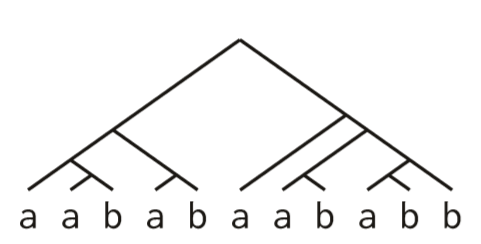
\includegraphics[width=0.7\linewidth]{figures/example.png}
	\caption{A Lyndon Tree for the Lyndon Word \texttt{aababaababb}}
	\label{fig:example}
\end{figure}
\end{frame}

\begin{frame}{Lyndon Tree}
	\par 每个节点对应的字符串都是原串$w$的一个子串$w[i...j]$。$[i...j]$被称为这个节点所对应的区间。我们用$lca([i...j])$来表示位置$i$到位置$j$之间的所有的叶子节点的LCA,即最近公共祖先。
	\pause
	\par 本质上是$ISA$数组的笛卡尔树。构造方法与之前计算Lyndon root的算法完全相同。可以在线性时间内构造。
\end{frame}

\begin{frame}{Lyndon Tree}
	\par \textbf{性质:} 若一个$w$的一个子串$w[i...j]$是Lyndon串,那么节点$\alpha = lca([i...j]) = [i_{\alpha}, j_{\alpha}]$,满足$i = i_{\alpha} \le j \le j_{\alpha}$。 若$w$是位置$i (i > 1)$开始的最长Lyndon串,那么节点$\alpha$一定是一个右儿子节点。
	\pause
	\par $w$的任意一个run的所有Lyndon root都会在$LTree_0(w)$或$LTree_1(w)$中的右儿子节点中出现。这里的$0$或$1$由\textbf{引理7}决定。
\end{frame}

\section{Applications of The Runs Theorem}

\subsection{Two-Period Queries}

\begin{frame}{Weak Periodicity Lemma}
	\par \textbf{引理:}若一个串$|S|$有$p$,$q$两个周期,且$p+q\le|S|$,则$\gcd(p,q)$也是$S$的周期。
	\pause
	\par \textbf{证明:}假设$p<q$。当$i\ge p$时$S[i]=S[i-p]=S[i-p+q]$;当$i<p$时$S[i]=S[i+q]=S[i+q-p]$。因此可以得到$q-p$也是$S$的周期。根据辗转相除法,$\gcd(p,q)$是$S$的周期。
	\pause
	\par \textbf{Periodicity Lemma:}若一个串$|S|$有$p$,$q$两个周期,且$p+q-\gcd(p,q)\le|S|$,则$\gcd(p,q)$也是$S$的周期。
	\pause
	\par 以下把Weak Periodicity Lemma简写为WPL。
\end{frame}

\begin{frame}{Two-Period Queries}
	\par \textbf{问题:}设计数据结构,支持快速查询母串$S$的某个子串是否有不超过长度一半的周期,如果有则求出最小周期。
	\pause
	\par \textbf{定义:}$exrun(i,j)$为满足$i'\le i,j'\ge j,p\le(j-i+1)/2$的一个run$(i',j',p)$。根据WPL,如果$exrun$存在则一定唯一。
	\pause
	\par \textbf{做法:}根据上面的定义,对$S[i...j]$的查询就等价于找到$exrun(i,j)$。我们先构造出$LTree_0(S)$和$LTree_1(S)$。算法为:令$a_0=lca_0\left(\big[i...\lceil(i+j)/2\rceil\big]\right)$,$a_1=lca_1\left(\big[i...\lceil(i+j)/2\rceil\big]\right)$,并判断它们的右儿子对应的run是否满足条件。
\end{frame}

\begin{frame}{Two-Period Queries}
	\par 假设$exrun(i,j)=r=(i',j',p)$,那么由于$p\leq(j-i+1)/2$,一定有一个Lyndon root $\lambda=[i_{\lambda}...j_{\lambda}]$包含$\lceil(j-i+1)/2\rceil$这个位置。根据Lyndon Tree的性质,这个Lyndon root在$LTree_{\ell}(S)$中作为某个节点的右儿子出现。
	\pause
	\par 这时我们有$a_{\ell}$的长度$>p$,且它同样包含$\lceil(j-i+1)/2\rceil$这个位置,因此$a_{\ell}$是$\lambda$的祖先。若它的右儿子$\beta=[i_{\beta}...j_{\beta}]\neq\lambda$,则$\beta$也是$\lambda$的祖先。因为$\lambda$和$\beta$都是右儿子,可以得到$i\leq i_{\beta}<i_{\lambda}$。
	\pause
	\par 若$j_{\beta}\le j$则$S[i_{\beta}...j_{\beta}]$有周期$p$,与它是Lyndon Word矛盾。若$j_{\beta}>j$可以发现$S[i_{\lambda}...j_{\beta}]<_{\ell}S[i_{\beta}...j_{\beta}]$,同样与它是Lyndon Word矛盾。
	\par 上述矛盾表明我们的算法是正确的。
\end{frame}

\begin{frame}{Two-Period Queries}
	\par \textbf{扩展:}更一般的Period Queries需要用到一种叫做基本子串字典的数据结构(Dictionary of Basic Factors),它可以做到$O(|S|\log|S|)$预处理,每次查询$O(\log|S|)$。这一数据结构基于后缀数组的倍增算法,在2017年金策的冬令营讲课中提到。
	\pause
	\par 另外,由于Lyndon Tree和后缀数组的笛卡尔树结构相同,维护Lyndon Tree可以转化为维护后缀数组。如果结合后缀平衡树等经典数据结构,可以把Two-Period Queries进行一定程度上的推广(如:树上)。
\end{frame}

\subsection{Primitive Squares}

\begin{frame}{串串划分(简化)\footnote{来源:杨骏昭的集训队互测题}}
	\par \textbf{问题:}给定一个串S,求把它划分为若干个循环串的方案数。若一个串$S$的最小周期$p$是$|S|$的真因数,则称$S$为循环串。$|S|\le10^6$
	\pause
	\par \textbf{做法:}首先可以设计简单的递推:$f(i)$表示$S[1...i]$的划分方案数。那么有$f(i)=\sum_{j=0}^{i-1}f(j)\cdot[S[i...j]\texttt{是循环串}]$。不过即使我们能快速判断每个串是否是循环串,这个递推的复杂度也是$O(|S|^2)$的。如何优化转移?
	\pause
	\par 首先,对于每个循环串,显然可以只在最小周期处考虑。我们把状态修改为:$f(i,p)$表示$S[1...i]$的划分,且最后一个划分的最小周期为$p$的方案数。这样,我们的转移就有两种方向:加入一个新的循环串;扩展当前循环串一个周期。为了不重复计数,我们强制新的循环串的最小周期为长度的一半。这个转移可以$O(1)$进行,因此我们只需要计算状态数。
	\pause
	\par \textbf{定义:}若串$S$的最小周期为$|S|/2$则称$S$为一个primitive square。注意由于WPL,这样的定义没有问题。
\end{frame}

\begin{frame}{串串划分(简化)}
	\par \textbf{引理:}若非空串$S,T$满足$SS$是$TT$的前缀,且$2|S|>|T|$,则$|T|-|S|$是$S$的周期。
	\par 此引理画图自证不难。
	\par \textbf{引理:}若非空串$u,v,w$满足$uu$是$vv$的前缀,$vv$是$ww$的前缀,且$uu$是primitive square,则$|u|+|v|\le|w|$。
	\pause
	\par \textbf{证明:}若$|w|\ge2|v|\ge|u|+|v|$则已证完。因此假设$|w|<2|v|$,并假设$|u|+|v|>|w|$,则$|w|-|v|$是$u$和$v$的周期。
	\pause
	\par 若$2|u|\le|v|$,则$|w|-|v|<|u|$是$uu$的周期,和primitive square的定义矛盾。
\end{frame}

\begin{frame}{串串划分(简化)}
	\par \textbf{证明:}考虑$2|u|>|v|$的情况。此时$|u|$和$|w|-|v|$都是$v$的周期,由于$u$不是周期串,意味着WPL不能使用在$v$串上,也就是$|u|+|w|>2|v|$。
	\pause
	\par 令$w=vs_1$,$u=s_1s_3$,$v=ws_2=s_1s_3s_2$。根据上面的推论,$|s_2|<|s_1|$。考虑串$s_3s_2$,它有周期$|s_2|$。由于$|s_1|$是$u$的周期,可得$s_3s_2$是$u$的前缀,这意味着$|s_3|$也是它的周期。根据WPL,$r=\gcd(|s_2|,|s_3|)$是它的周期。而$|s_2|$本身同时是$u$的周期,因此可得$r$是$u$的周期。
	\pause
	\par 接着考虑串$u=s_1s_3$。它的周期有$|s_1|$和$r$,而$r\le|s_3|$,根据WPL,$r'=\gcd(r,|s_1|)$也是$u$的周期。然而$|s_1|$和$|s_3|$都是$r'$的倍数,这表示$uu$也有周期$r'$,矛盾。
	\qed
	\pause
	\par 引理的一个显然的推论是,一个串$S$中primitive square的个数不超过$O(|S|\log|S|)$。
\end{frame}

\begin{frame}
	\par 有了之前的引理,最终剩下的问题就是如何找出所有的primitive squares。由于每个primitive square一定属于恰好一个和它的周期对应的run的一部分,我们只要求出所有的run,并对每个run暴力即可。
	\pause
	\par 综上,我们得到了一个$O(n\log n)$的做法。不难发现,对于大部分和周期串相关的问题,都可以对每个周期串在最后一个primitive square处考虑并简化状态数。
	\pause
\end{frame}

\begin{frame}
\begin{figure}[h]%%图片
	\centering 
	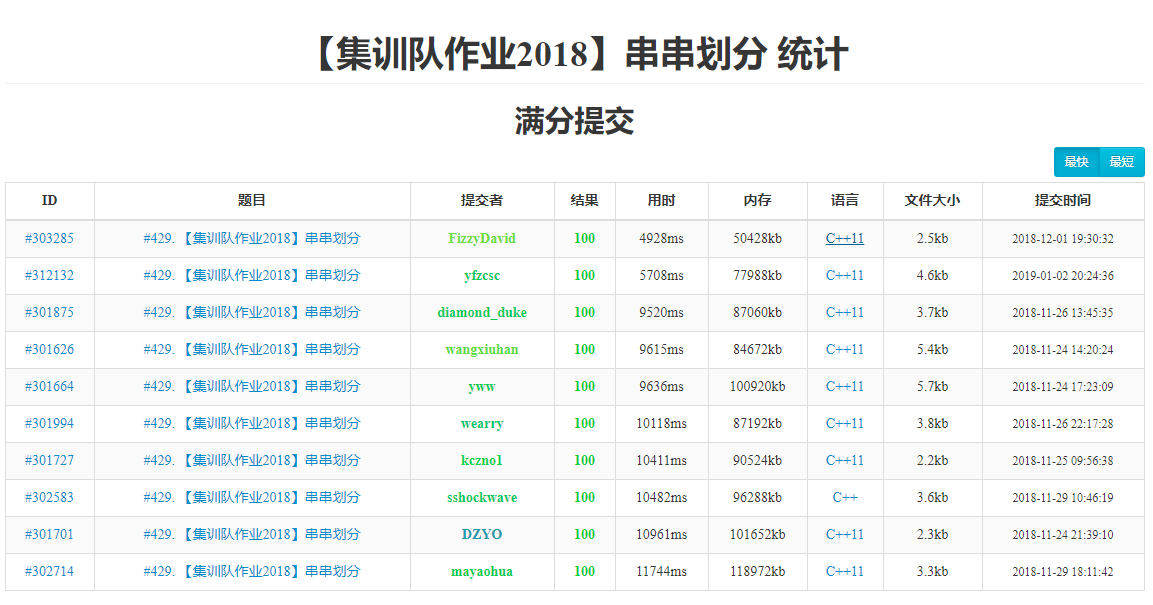
\includegraphics[width=0.7\linewidth]{figures/runtime.png}
\end{figure}
	\par 可以发现,primitive square和run是密切相关的,知道一个就能求出另一个。在杨骏昭的题解中给出的是一个不基于Lyndon Word任何性质的做法。而这里的做法的优势在于代码复杂度和用时都较小。
\end{frame}

\section{Conclusion}

\subsection{Summary}

\begin{frame}{Summary}
    \par - Runs and The Runs Theorem - 徐翊轩
	\pause
    \par - How to Compute Runs and Lyndon Tree - 杨骏昭
	\pause
    \par - Applications of The Runs Theorem - 陈孙立
\end{frame}

\begin{frame}{参考文献}
	\par \textbf{[1]} Hideo Bannai, Tomohiro I, Shunsuke Inenaga, Yuto Nakashima, Masayuki Takeda, Kazuya Tsuruta, \emph{The “Runs” Theorem}
	\par \textbf{[2]} Maxime Crochemore, Lu´ıs M. S. Russo, \emph{Cartesian trees and Lyndon trees}
\end{frame}

\subsection{Thanks}

\begin{frame}{Thanks}
    \par 谢谢大家。
\end{frame}

\end{document}
